\documentclass[border=4pt]{standalone}
\usepackage[T1]{fontenc}
\usepackage{helvet}
\renewcommand{\familydefault}{\sfdefault}
\usepackage{graphicx}
\usepackage{caption}
\usepackage{amsmath}
\captionsetup{font={sf,footnotesize},labelfont={sf,bf,footnotesize},justification=justified,singlelinecheck=false}
\begin{document}
\setcounter{figure}{1}
\begin{minipage}{7.20in}
\centering
\begin{figure}[htbp]
    \centering
    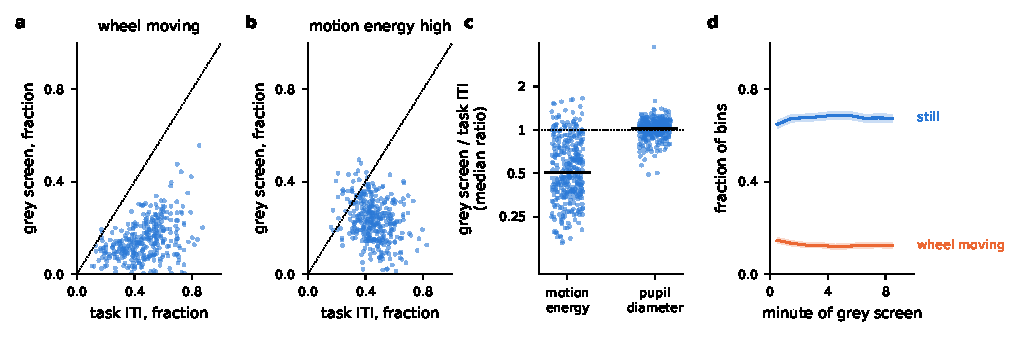
\includegraphics[width=\linewidth]{fig2_movement_panels.pdf}
    \caption{\textbf{a} Fraction of 50 ms bins with wheel movement in the grey-screen period against task inter-trial intervals (feedback + 1.5 s to next stimulus onset $-$ 0.5 s) of the same session; dots are the 338 sessions with wheel data in both. \textbf{b} Same for motion energy above the session's 60th percentile (361 sessions with motion energy). \textbf{c} Median motion energy and pupil diameter in the grey-screen period relative to task ITIs; bars are medians over sessions. \textbf{d} Time course over the grey-screen period in whole minutes (the first second is skipped, so a 600 s period gives 9 full minutes; 300 s sessions contribute to the first 4): fraction of still bins and of bins with wheel movement, mean over sessions with 95\% CI.}
    \label{fig:grey_movement}
\end{figure}
\end{minipage}
\end{document}
